\documentclass[12pt]{article}

\usepackage[spanish]{babel}
\usepackage{hyperref}
\usepackage{graphicx}
\usepackage{listings}
\usepackage{color}
\usepackage{multicol}
\usepackage{amssymb}
\usepackage{enumitem}
\usepackage{here}
\usepackage{dsfont}
\usepackage{amsmath}
\usepackage{tipa}
\usepackage{float}
\spanishdecimal{.}

\title{Matemáticas para las Ciencias Aplicadas I}
\title{
	Tercera Lista de Problemas \\
	\textbf{Primera  Parte} \\
	\vspace{1ex}
	\large Matemáticas para las Ciencias Aplicadas I \\
	Facultad de Ciencias, UNAM}

\date{\today}

\author{Flores Morán Julieta Melina \\ Zarco Romero José Antonio}

\begin{document}

\maketitle

%% De la sección 3.2: ejercicios 38 y 57.
%% De la sección 3.3: ejercicios 54, 70, 76 y 83.
%% De la sección 3.4: ejercicios 23, 36, 45 y 47.
 %% De la sección 3.6: ejercicios 58, 63 y 65

%% 3.2 -------------------------------------------------------------------------------------------------------------------------------------------------------------------------------------------------------------------------------
\section{Sección 3.2 \\ Derivadas De Funciones Logarítmicas}
% 38 -------------------------------------------------------------------------------------------------------------
\subsection{Ejercicio 38} name \\

Encuentre $dy/dx$ usando diferenciación logarítmica.
\[
y=\frac{\sin{x}\cos{x}\tan^3{x}}{\sqrt{x}}
\]
\begin{equation*}
  \begin{split}
  \ln(y)
  &= \ln(\sin{x}\cos{x}\tan^3{x})-\ln(\sqrt{x}) \\
  &= \ln(\sin{x})+\ln(\cos{x})+\ln(\tan^3{x})-\ln \left(x^{\frac{1}{2}}\right) \\
  &= \ln(\sin{x})+\ln(\cos{x})+3\ln(\tan{x})-\frac{1}{2}\ln x \\
  \frac{1}{y}\frac{dy}{dy}
  &= \frac{\cos{x}}{\sin{x}} + \frac{-\sin{x}}{\cos{x}} + \frac{3\sec^2{x}}{\tan{x}} - \frac{1}{2x} \\
  \frac{dy}{dy}
  &= y \left[ \cot{x}-\tan{x} + \frac{3\sec^2{x}}{\tan{x}} - \frac{1}{2x} \right] \\
  \therefore \frac{dy}{dy}
  &= \frac{\sin{x}\cos{x}\tan^3{x}}{\sqrt{x}}
  \left[ \cot{x}-\tan{x} + \frac{3\sec^2{x}}{\tan{x}} - \frac{1}{2x} \right] \\
  \end{split}
\end{equation*}

% 57 -------------------------------------------------------------------------------------------------------------
\subsection{Ejercicio 57} name \\

Sea $p$ el número de paramecios en una solución nutritiva $t$ días después del inicio de un experimento, y supongamos que $p$ es definido implícitamente como una función de $t$ por la ecuación
\[
0 = \ln p + 0.83 − \ln(2.3 − 0.0046p) − 2.3t
\]
Utilice la diferenciación implícita para demostrar que la tasa de cambio de $p$ con respecto a $t$ satisface la ecuación
\[
\frac{dp}{dt} = 0.0046p(500-p)
\]
\begin{equation*}
  \begin{split}
    \ln p - \ln(2.3 − 0.0046p)
    &= 2.3t -0.83 \\
    \frac{1}{p}\frac{dp}{dt}+\frac{0.0046}{2.3-0.0046p}\frac{dp}{dt}
    &= 2.3 \\
    \frac{dp}{dt}\left[\frac{1}{p}+\frac{0.0046}{2.3-0.0046p}\right]
    &= 2.3 \\
    \frac{dp}{dt}\left[\frac{2.3-0.0046p+ 0.0046p}{p(2.3-0.0046p)}\right]
    &= 2.3 \\
    \frac{dp}{dt}\left[\frac{2.3}{2.3p-0.0046p^2}\right]
    &= 2.3 \\
    \frac{dp}{dt}
    &= 2.3\left[\frac{2.3p-0.0046p^2}{2.3}\right] \\
    &= 2.3p-0.0046p^2 \\
    \therefore \frac{dp}{dt}
    &= 0.0046p(500-p)
  \end{split}
\end{equation*}

%% 3.3 -----------------------------------------------------------------------------------------------------------------------------------------------------------------------------------------------------------------------------
\section{Sección 3.3 \\ Derivadas De Funciones Trigonométricas Exponenciales E Inversas} 
% 54 -------------------------------------------------------------------------------------------------------------
\subsection{Ejercicio 54} name \\

Encuentre $\frac{dy}{dx}$.
\[
y=x^2(\sin^{-1}{x})^3
\]
\begin{equation*}
  \begin{split}
    \frac{dy}{dx}
    &= \left[x^2\cdot \frac{d}{dx}(\sin^{-1}{x})^3 \right] + \left[(\sin^{-1}{x})^3\cdot \frac{d}{dx}x^2\right] \\
    &= \left\lbrace x^2\cdot \left[3(\sin^{-1}{x})^2\cdot \frac{d}{dx}(\sin^{-1}{x}) \right] \right\rbrace + \left[(\sin^{-1}{x})^3\cdot 2x\right] \\
    &= \left\lbrace x^2\cdot \left[3(\sin^{-1}{x})^2\cdot \frac{1}{\sqrt{1-x^2}} \right] \right\rbrace + \left[2x(\sin^{-1}{x})^3\right] \\
    &= \left\lbrace x^2\cdot \left[ \frac{3(\sin^{-1}{x})^2}{\sqrt{1-x^2}} \right] \right\rbrace + 2x(\sin^{-1}{x})^3 \\
    \therefore
    \frac{dy}{dx}
    &= \frac{3x^2(\sin^{-1}{x})^2}{\sqrt{1-x^2}} + 2x(\sin^{-1}{x})^3 \\
  \end{split}
\end{equation*}

% 70 -------------------------------------------------------------------------------------------------------------
\subsection{Ejercicio 70} name \\

Sea $f(x)=\frac{exp(4-x^2)}{x}$, $x>0$.
\begin{enumerate}
\item Demuestre que $f$ es uno a uno.
\item Sea $g(x)=f^-1(x)$ y defina $F(X)=f([g(x)]^2)$. Encuentre $F'\left(\frac{1}{2}\right)$
\end{enumerate}

% 76 -------------------------------------------------------------------------------------------------------------
\subsection{Ejercicio 76} name \\

Supongamos que la población de bacterias dependientes de oxígeno en un estanque se modela mediante la ecuación
\[
P(t)=\frac{60}{5+7e^{-t}}
\]
donde $P(t)$ es la población (en miles de millones) $t$ días después de una observación inicial en el momento $t = 0$.
\begin{enumerate}
\item Utilice una herramienta gráfica para representar gráficamente la función $P(t)$.
\item Explique con palabras qué le sucede a la población a lo largo del tiempo. Comprueba tu conclusión encontrando $\lim_{t \to +\infty} P(t)$.
\item En palabras, ¿qué sucede con la \textit{tasa} de crecimiento de la población a lo largo del tiempo? Comprueba tu conclusión graficando $P'(t)$.
\end{enumerate}

% 83 -------------------------------------------------------------------------------------------------------------
\subsection{Ejercicio 83} name \\

Supongamos que un rodamiento  de bolas de acero se suelta dentro de una tina de fluido y comienza a hundirse. Según un modelo, la velocidad $v(t)$ (en $m/s$) del rodamiento de bolas $t$ segundos después de su liberación viene dada por la fórmula
\[
v(t)=\frac{9.8}{k}(1-e^{-kt})
\]
donde $k$ es una constante positiva que corresponde a la resistencia que ofrece el fluido contra el movimiento del rodamiento. (Cuanto menor sea el valor de $k$, más débil será la resistencia).
Para $t$ fijo, determine el valor límite de la velocidad cuando $k\rightarrow 0^+$ y dé una interpretación física del límite.
\begin{equation*}
  \begin{split}
    \lim_{k \to 0^+} v(t)
    &= \lim_{k \to 0^+} \left[ \frac{9.8}{k}(1-e^{-kt}) \right] \\
    &= 9.8 \lim_{k \to 0^+} \frac{1-e^{-kt}}{k} \\
    & \qquad \text{Aplicando la serie de MacLaurin, tenemos que:} \\
    &= 9.8 \lim_{k \to 0^+} \frac{1-
      \left(1+\frac{(-kt)}{1!}+\frac{(-kt)^2}{2!}+\frac{(-kt)^3}{3!}+\ldots \right)
    }{k} \\
    &= 9.8 \lim_{k \to 0^+} \frac{1-
      \left(1-kt+\frac{(kt)^2}{2!}-\frac{(kt)^3}{3!}+\ldots \right)
    }{k} \\
    &= 9.8 \lim_{k \to 0^+} \frac{kt-\frac{(kt)^2}{2!}+\frac{(kt)^3}{3!}-\ldots}{k} \\
    &= 9.8 \lim_{k \to 0^+} \left[ t-\frac{k(t)^2}{2!}+\frac{k^2t^3}{3!}-\ldots \right] \\
    &= 9.8 ( t-0+0-\ldots ) \\
    \therefore
    \lim_{k \to 0^+} v(t)
    &= 9.8 t \\
  \end{split}
\end{equation*}

Esto significa que si el fluido no ofrece resistencia, entonces la velocidad aumentará a una tasa constante de $9.8 m/s$.

%% 3.4 -----------------------------------------------------------------------------------------------------------------------------------------------------------------------------------------------------------------------------
\section{Sección 3.4 \\ Tasas Relacionadas} 
% 23 -------------------------------------------------------------------------------------------------------------
\subsection{Ejercicio 23} name \\

\begin{figure}[H]
\centering
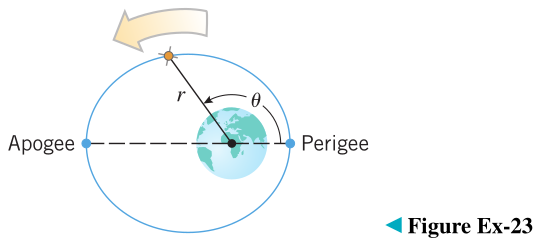
\includegraphics[width=0.6\textwidth]{../img/img_Lista3/23.png}
\end{figure}
Un satélite se encuentra en una órbita elíptica alrededor de la Tierra. Su distancia $r$ (en millas) desde el centro de la Tierra está dada por
\[
r=\frac{4995}{1+0.12\cos{\theta}}
\]
donde $\theta$ es el ángulo medido desde el punto de la órbita más cercano a la superficie de la Tierra (consulte la figura adjunta).
\begin{enumerate}
\item Encuentre la altitud del satélite en el \textit{\textbf{perigeo}} (el punto más cercano a la superficie de la Tierra) y en el \textit{\textbf{apogeo}} (el punto más alejado de la superficie de la Tierra). Utilice $3960 mi$ como radio de la Tierra.
\item En el instante en que $\theta$ es $120^{\circ}$, el ángulo $\theta$ aumenta a razón de $2.7^{\circ} /min$. Encuentre la altitud del satélite y la velocidad a la que cambia la altitud en este instante. Exprese la velocidad en unidades de $mi/min$.
\end{enumerate}

% 36 -------------------------------------------------------------------------------------------------------------
\subsection{Ejercicio 36} name \\

Un helicóptero de la policía vuela hacia el norte a $100 mi/h$ y a una altitud constante de $\frac{1}{2} mi$. A continuación, un automóvil viaja hacia el oeste por una carretera a $75 mi/h$. En el momento en que el helicóptero cruza la carretera, el automóvil se encuentra a 2 millas al este del helicóptero.
\begin{enumerate}
\item ¿A qué velocidad cambia la distancia entre el automóvil y el helicóptero en el momento en que el helicóptero cruza la carretera?
\item ¿La distancia entre el coche y el helicóptero aumenta o disminuye en ese momento?
\end{enumerate}

% 45 -------------------------------------------------------------------------------------------------------------
\subsection{Ejercicio 45} name \\

Un meteoro entra en la atmósfera terrestre y se quema a un ritmo que, en cada instante, es proporcional a su superficie. Suponiendo que el meteoro es siempre esférico, demuestre que el radio disminuye a un ritmo constante.

% 47 -------------------------------------------------------------------------------------------------------------
\subsection{Ejercicio 47} name \\

\begin{figure}[H]
\centering
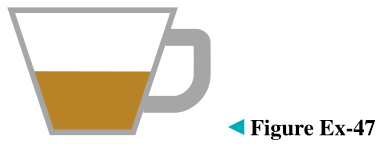
\includegraphics[width=0.4\textwidth]{../img/img_Lista3/47.png}
\end{figure}
Se vierte café a una velocidad uniforme de $20 cm^3/s$ en una taza cuyo interior tiene forma de cono truncado (consulte la figura adjunta). Si los radios superior e inferior de la taza son 4 cm y 2 cm y la altura de la taza es 6 cm, ¿con qué rapidez aumentará el nivel del café cuando el café esté a la mitad? [\textit{Sugerencia}: extienda la copa hacia abajo para formar un cono.]

%% 3.6 -----------------------------------------------------------------------------------------------------------------------------------------------------------------------------------------------------------------------------
\section{Sección 3.6 \\ La Regla De L'Hôpital; Formas Indeterminadas} 
% 58 -------------------------------------------------------------------------------------------------------------
\subsection{Ejercicio 58} name \\

Hay un mito que circula entre los estudiantes principiantes de cálculo que afirma que todas las formas indeterminadas de tipos $0^0,\infty^0$ y $1^{\infty}$ tienen valor 1 porque ''cualquier cosa elevada a cero es 1'' y ''1 elevado a cualquier potencia es 1''. La falacia es que $0^0,\infty^0$ y $1^{\infty}$ no son potencias de números, sino descripciones de límites. Los siguientes ejemplos, sugeridos por el Prof. Jack Staib de la Universidad de Drexel, muestran que estas formas indeterminadas pueden tener cualquier valor real positivo.
valor:
\begin{enumerate}[label=(\alph*)]
\item $\lim_{x \to 0^+} [x^{(\ln a)/(1+\ln x)}]=a \qquad$ (forma $0^0$)
\item $\lim_{x \to +\infty} [x^{(\ln a)/(1+\ln x)}]=a \qquad$ (forma $\infty^0$)
\item $\lim_{x \to 0} [(x+1)^{(\ln a)/x}]=a \qquad$ (forma $1^{\infty}$)
\end{enumerate}
Verifique estos resultados.

% 63 -------------------------------------------------------------------------------------------------------------
\subsection{Ejercicio 63} name \\
% 65 -------------------------------------------------------------------------------------------------------------
\subsection{Ejercicio 65} name \\

\end{document}
